%% The union API — COLUMN variant. Vertical stack, bidirectional arrows (the
%% same path carries payloads down and received data back up). Tight.
\documentclass[tikz,border=4pt]{standalone}
\usepackage{xcolor}
%% Shared look for the UnionLabs system figures. \input by each fig-*.tex so a
%% colour or a corner radius is changed in one place.
\usetikzlibrary{positioning,arrows.meta,fit,backgrounds,calc}

\definecolor{uCode}{HTML}{1F6F5C}     % the experimenter's own code
\definecolor{uApi}{HTML}{6B4BA8}      % the contract / ARQ layer
\definecolor{uPhy}{HTML}{2E5E9E}      % transports / DSP
\definecolor{uRadio}{HTML}{B4700F}    % hardware
\definecolor{uShare}{HTML}{8A2E4D}    % the shared workspace

\tikzset{
  blk/.style={draw, rounded corners=2pt, align=center, font=\small,
              minimum height=8mm, inner sep=3pt, fill=black!2},
  code/.style={blk, draw=uCode, thick, fill=uCode!6},
  api/.style={blk, draw=uApi, very thick, fill=uApi!7},
  phy/.style={blk, draw=uPhy, thick, fill=uPhy!6},
  radio/.style={blk, draw=uRadio, thick, fill=uRadio!8},
  share/.style={blk, draw=uShare, thick, fill=uShare!6},
  stage/.style={blk, minimum height=9.5mm, font=\scriptsize, text width=16mm,
                inner sep=2pt},
  flow/.style={-{Latex[length=2mm]}, thick},
  back/.style={-{Latex[length=2mm]}, thick, densely dashed},
  % labels that sit ON an arrow: opaque, so the line never strikes the text
  onarrow/.style={font=\scriptsize\itshape, fill=white, inner sep=1.5pt},
  lbl/.style={font=\scriptsize\itshape, inner sep=1pt},
  note/.style={font=\scriptsize, align=left, inner sep=1pt},
  legend/.style={draw, minimum width=3mm, minimum height=3mm, inner sep=0pt},
}
\newcommand{\mono}[1]{{\ttfamily\footnotesize #1}}
\newcommand{\monos}[1]{{\ttfamily\scriptsize #1}}

\begin{document}
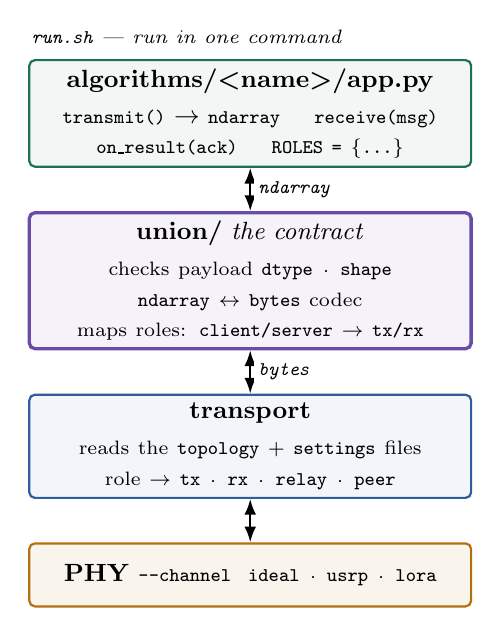
\begin{tikzpicture}[x=1mm, y=1mm,
  duplex/.style={{Latex[length=2mm]}-{Latex[length=2mm]}, thick}]

\node[code, text width=54mm] (app) at (0,0)
  {\textbf{algorithms/\textless name\textgreater/app.py}\\[2pt]
   \monos{transmit()} $\rightarrow$ \monos{ndarray} \quad \monos{receive(msg)}\\
   \monos{on\_result(ack)} \quad \monos{ROLES = \{...\}}};
\node[lbl, above=1.5mm of app.north west, anchor=south west]
  {\monos{run.sh} --- run in one command};

\node[api, text width=54mm, below=5.5mm of app] (api)
  {\textbf{union/} \emph{the contract}\\[2pt]
   {\scriptsize checks payload \monos{dtype · shape}}\\
   {\scriptsize \monos{ndarray} $\leftrightarrow$ \monos{bytes} codec}\\
   {\scriptsize maps roles: \monos{client/server} $\rightarrow$ \monos{tx/rx}}};

\node[phy, text width=54mm, below=5.5mm of api] (tr)
  {\textbf{transport}\\[2pt]
   {\scriptsize reads the \monos{topology} + \monos{settings} files}\\
   {\scriptsize role $\rightarrow$ \monos{tx · rx · relay · peer}}};

\node[radio, text width=54mm, below=5.5mm of tr] (phy)
  {\textbf{PHY} \monos{--channel}\ \ \monos{ideal · usrp · lora}};

\draw[duplex] (app) -- node[onarrow, right=1pt] {\monos{ndarray}} (api);
\draw[duplex] (api) -- node[onarrow, right=1pt] {\monos{bytes}} (tr);
\draw[duplex] (tr) -- (phy);

\end{tikzpicture}
\end{document}
